% Options for packages loaded elsewhere
\PassOptionsToPackage{unicode}{hyperref}
\PassOptionsToPackage{hyphens}{url}
%
\documentclass[
]{article}
\usepackage{amsmath,amssymb}
\usepackage{iftex}
\ifPDFTeX
  \usepackage[T1]{fontenc}
  \usepackage[utf8]{inputenc}
  \usepackage{textcomp} % provide euro and other symbols
\else % if luatex or xetex
  \usepackage{unicode-math} % this also loads fontspec
  \defaultfontfeatures{Scale=MatchLowercase}
  \defaultfontfeatures[\rmfamily]{Ligatures=TeX,Scale=1}
\fi
\usepackage{lmodern}
\ifPDFTeX\else
  % xetex/luatex font selection
\fi
% Use upquote if available, for straight quotes in verbatim environments
\IfFileExists{upquote.sty}{\usepackage{upquote}}{}
\IfFileExists{microtype.sty}{% use microtype if available
  \usepackage[]{microtype}
  \UseMicrotypeSet[protrusion]{basicmath} % disable protrusion for tt fonts
}{}
\makeatletter
\@ifundefined{KOMAClassName}{% if non-KOMA class
  \IfFileExists{parskip.sty}{%
    \usepackage{parskip}
  }{% else
    \setlength{\parindent}{0pt}
    \setlength{\parskip}{6pt plus 2pt minus 1pt}}
}{% if KOMA class
  \KOMAoptions{parskip=half}}
\makeatother
\usepackage{xcolor}
\usepackage[margin=1in]{geometry}
\usepackage{color}
\usepackage{fancyvrb}
\newcommand{\VerbBar}{|}
\newcommand{\VERB}{\Verb[commandchars=\\\{\}]}
\DefineVerbatimEnvironment{Highlighting}{Verbatim}{commandchars=\\\{\}}
% Add ',fontsize=\small' for more characters per line
\usepackage{framed}
\definecolor{shadecolor}{RGB}{248,248,248}
\newenvironment{Shaded}{\begin{snugshade}}{\end{snugshade}}
\newcommand{\AlertTok}[1]{\textcolor[rgb]{0.94,0.16,0.16}{#1}}
\newcommand{\AnnotationTok}[1]{\textcolor[rgb]{0.56,0.35,0.01}{\textbf{\textit{#1}}}}
\newcommand{\AttributeTok}[1]{\textcolor[rgb]{0.13,0.29,0.53}{#1}}
\newcommand{\BaseNTok}[1]{\textcolor[rgb]{0.00,0.00,0.81}{#1}}
\newcommand{\BuiltInTok}[1]{#1}
\newcommand{\CharTok}[1]{\textcolor[rgb]{0.31,0.60,0.02}{#1}}
\newcommand{\CommentTok}[1]{\textcolor[rgb]{0.56,0.35,0.01}{\textit{#1}}}
\newcommand{\CommentVarTok}[1]{\textcolor[rgb]{0.56,0.35,0.01}{\textbf{\textit{#1}}}}
\newcommand{\ConstantTok}[1]{\textcolor[rgb]{0.56,0.35,0.01}{#1}}
\newcommand{\ControlFlowTok}[1]{\textcolor[rgb]{0.13,0.29,0.53}{\textbf{#1}}}
\newcommand{\DataTypeTok}[1]{\textcolor[rgb]{0.13,0.29,0.53}{#1}}
\newcommand{\DecValTok}[1]{\textcolor[rgb]{0.00,0.00,0.81}{#1}}
\newcommand{\DocumentationTok}[1]{\textcolor[rgb]{0.56,0.35,0.01}{\textbf{\textit{#1}}}}
\newcommand{\ErrorTok}[1]{\textcolor[rgb]{0.64,0.00,0.00}{\textbf{#1}}}
\newcommand{\ExtensionTok}[1]{#1}
\newcommand{\FloatTok}[1]{\textcolor[rgb]{0.00,0.00,0.81}{#1}}
\newcommand{\FunctionTok}[1]{\textcolor[rgb]{0.13,0.29,0.53}{\textbf{#1}}}
\newcommand{\ImportTok}[1]{#1}
\newcommand{\InformationTok}[1]{\textcolor[rgb]{0.56,0.35,0.01}{\textbf{\textit{#1}}}}
\newcommand{\KeywordTok}[1]{\textcolor[rgb]{0.13,0.29,0.53}{\textbf{#1}}}
\newcommand{\NormalTok}[1]{#1}
\newcommand{\OperatorTok}[1]{\textcolor[rgb]{0.81,0.36,0.00}{\textbf{#1}}}
\newcommand{\OtherTok}[1]{\textcolor[rgb]{0.56,0.35,0.01}{#1}}
\newcommand{\PreprocessorTok}[1]{\textcolor[rgb]{0.56,0.35,0.01}{\textit{#1}}}
\newcommand{\RegionMarkerTok}[1]{#1}
\newcommand{\SpecialCharTok}[1]{\textcolor[rgb]{0.81,0.36,0.00}{\textbf{#1}}}
\newcommand{\SpecialStringTok}[1]{\textcolor[rgb]{0.31,0.60,0.02}{#1}}
\newcommand{\StringTok}[1]{\textcolor[rgb]{0.31,0.60,0.02}{#1}}
\newcommand{\VariableTok}[1]{\textcolor[rgb]{0.00,0.00,0.00}{#1}}
\newcommand{\VerbatimStringTok}[1]{\textcolor[rgb]{0.31,0.60,0.02}{#1}}
\newcommand{\WarningTok}[1]{\textcolor[rgb]{0.56,0.35,0.01}{\textbf{\textit{#1}}}}
\usepackage{graphicx}
\makeatletter
\def\maxwidth{\ifdim\Gin@nat@width>\linewidth\linewidth\else\Gin@nat@width\fi}
\def\maxheight{\ifdim\Gin@nat@height>\textheight\textheight\else\Gin@nat@height\fi}
\makeatother
% Scale images if necessary, so that they will not overflow the page
% margins by default, and it is still possible to overwrite the defaults
% using explicit options in \includegraphics[width, height, ...]{}
\setkeys{Gin}{width=\maxwidth,height=\maxheight,keepaspectratio}
% Set default figure placement to htbp
\makeatletter
\def\fps@figure{htbp}
\makeatother
\setlength{\emergencystretch}{3em} % prevent overfull lines
\providecommand{\tightlist}{%
  \setlength{\itemsep}{0pt}\setlength{\parskip}{0pt}}
\setcounter{secnumdepth}{5}
% Load necessary packages
\usepackage{amsmath}    % For advanced math typesetting
\usepackage{graphicx}   % For including images
\usepackage{hyperref}   % For hyperlinks
\usepackage{geometry}   % For setting page dimensions
\usepackage{fancyhdr}   % For custom headers and footers
\usepackage{setspace}   % For setting line spacing

% Set page dimensions
\geometry{
  a4paper,
  left=25mm,
  right=25mm,
  top=25mm,
  bottom=25mm
}

% Custom header and footer
\pagestyle{fancy}
\fancyhf{}
\fancyhead[L]{\leftmark}
\fancyhead[R]{\thepage}

% Custom commands
\newcommand{\HRule}{\rule{\linewidth}{0.5mm}}

% Set line spacing
\setstretch{1.5}

% Additional settings
\hypersetup{
  colorlinks=true,
  linkcolor=blue,
  filecolor=magenta,
  urlcolor=cyan,
  pdftitle={Your Document Title},
  pdfpagemode=FullScreen,
}
\ifLuaTeX
  \usepackage{selnolig}  % disable illegal ligatures
\fi
\IfFileExists{bookmark.sty}{\usepackage{bookmark}}{\usepackage{hyperref}}
\IfFileExists{xurl.sty}{\usepackage{xurl}}{} % add URL line breaks if available
\urlstyle{same}
\hypersetup{
  pdftitle={Lecture 8: Multiple Regression},
  pdfauthor={Dr Peter E McKenna},
  hidelinks,
  pdfcreator={LaTeX via pandoc}}

\title{Lecture 8: Multiple Regression}
\usepackage{etoolbox}
\makeatletter
\providecommand{\subtitle}[1]{% add subtitle to \maketitle
  \apptocmd{\@title}{\par {\large #1 \par}}{}{}
}
\makeatother
\subtitle{C91AR: Advanced Statistics using R}
\author{Dr Peter E McKenna}
\date{2025-03-11}

\begin{document}
\maketitle

{
\setcounter{tocdepth}{2}
\tableofcontents
}
\hypertarget{setup-code}{%
\section{Setup code}\label{setup-code}}

\begin{Shaded}
\begin{Highlighting}[]
\CommentTok{\# change output format}
\FunctionTok{options}\NormalTok{(}\AttributeTok{scipen =} \DecValTok{999}\NormalTok{)}

\CommentTok{\# set the seed}
\FunctionTok{set.seed}\NormalTok{(}\DecValTok{453}\NormalTok{)}

\CommentTok{\# load packages}
\NormalTok{pacman}\SpecialCharTok{::}\FunctionTok{p\_load}\NormalTok{(corrr,}
\NormalTok{               tidyverse,}
\NormalTok{               psych,}
\NormalTok{               tidyplots)}
\end{Highlighting}
\end{Shaded}

\hypertarget{content-for-today}{%
\section{Content for today}\label{content-for-today}}

\begin{itemize}
\tightlist
\item
  Multiple regression formula
\item
  Worked example using the ``grades.csv'' dataset from PsyTeachR
\item
  The \texttt{predict} function
\item
  Partial effects
\item
  Standardising coefficients
\item
  Model comparison
\end{itemize}

\hypertarget{getting-started-with-multiple-regression}{%
\section{Getting started with Multiple
regression}\label{getting-started-with-multiple-regression}}

The general model for single-level data with \(m\) predictors is:

\[Y_i = \beta_0 + \beta_1 X_{1i} + \beta_2 X_{2i} + ... \beta_mX_{mi} + e_i\]

\begin{itemize}
\item
  Key assumption is that the model residuals are normally distributed.
\item
  Predictor variables \(X\) can be either categorical or continuous, as
  well as interactions between predictors.
\item
  \(e_i\) = difference between the predicted and the observed value of
  \(Y\) for the \emph{i}th participant.
\item
  The relationship is planar, i.e., can be described by a flat surface.
\item
  Error variable is independent of the predictor values.
\end{itemize}

\hypertarget{coefficients}{%
\section{Coefficients}\label{coefficients}}

\begin{itemize}
\tightlist
\item
  In multiple regression you will have \(m+1\) regression coefficients;
  one for the intercept (\(\beta_0\)), and one for each predictor
  (\(X_m\)).
\item
  Each \(\beta_{h}\) value (coefficient associated with the \(h^{th}\)
  independent variable) is understood as the partial effect of
  \(\beta_{h}\) holding constant all other predictors.
\item
  In other words, a partial effect of a coefficient in multiple
  regression refers to the effect of a particular IV on the DV, whilst
  holding all other IVs constant.
\item
  Response variable (\(Y\)) is predicted from a combination of all of
  the variables multiplied by their respective coefficients, plus a
  residual term.
\end{itemize}

\hypertarget{what-is-the-purpose-of-multiple-regression}{%
\section{What is the purpose of multiple
regression?}\label{what-is-the-purpose-of-multiple-regression}}

\begin{itemize}
\tightlist
\item
  \textbf{To identify a linear combination of predictors that exhibits
  the highest correlation with the response variable.}
\end{itemize}

\hypertarget{a-worked-example-using-the-grades.csv-dataset}{%
\section{\texorpdfstring{A worked example using the \texttt{grades.csv}
dataset}{A worked example using the grades.csv dataset}}\label{a-worked-example-using-the-grades.csv-dataset}}

\begin{itemize}
\tightlist
\item
  How do you get a good grade in statistics?
\end{itemize}

\begin{Shaded}
\begin{Highlighting}[]
\NormalTok{grades }\OtherTok{\textless{}{-}} 
  \FunctionTok{read\_csv}\NormalTok{(}\StringTok{"data\_tidy/grades.csv"}\NormalTok{, }
           \AttributeTok{col\_types =} \StringTok{"ddii"}\NormalTok{)}

\NormalTok{grades}
\end{Highlighting}
\end{Shaded}

\begin{verbatim}
## # A tibble: 100 x 4
##    grade   GPA lecture nclicks
##    <dbl> <dbl>   <int>   <int>
##  1  2.40 1.13        6      88
##  2  3.67 0.971       6      96
##  3  2.85 3.34        6     123
##  4  1.36 2.76        9      99
##  5  2.31 1.02        4      66
##  6  2.58 0.841       8      99
##  7  2.69 4           5      86
##  8  3.05 2.29        7     118
##  9  3.21 3.39        9      98
## 10  2.24 3.27       10     115
## # i 90 more rows
\end{verbatim}

\hypertarget{metadata}{%
\subsection{Metadata}\label{metadata}}

\begin{itemize}
\tightlist
\item
  N=100 statistics students
\item
  \texttt{grade} = final course grade
\item
  \texttt{lecture} = number of lectures attended; an integer from 0:10
\item
  \texttt{nclicks} = number of times the students clicked to download
  online materials
\item
  \texttt{GPA} = grade point average prior to taking the course; ranging
  from 0 (fail) to 4 (best possible grade)
\end{itemize}

\hypertarget{examine-pairwise-correlations}{%
\subsection{Examine pairwise
correlations}\label{examine-pairwise-correlations}}

\begin{Shaded}
\begin{Highlighting}[]
\CommentTok{\# Examine pairwise correlations}
\NormalTok{grades }\SpecialCharTok{|\textgreater{}}
  \FunctionTok{correlate}\NormalTok{() }\SpecialCharTok{|\textgreater{}}
  \FunctionTok{shave}\NormalTok{() }\SpecialCharTok{|\textgreater{}} 
  \FunctionTok{fashion}\NormalTok{() }\CommentTok{\# shave \& fashion tidy up the output}
\end{Highlighting}
\end{Shaded}

\begin{verbatim}
##      term grade  GPA lecture nclicks
## 1   grade                           
## 2     GPA   .25                     
## 3 lecture   .24  .44                
## 4 nclicks   .16  .30     .36
\end{verbatim}

\begin{center}\rule{0.5\linewidth}{0.5pt}\end{center}

\begin{Shaded}
\begin{Highlighting}[]
\FunctionTok{pairs}\NormalTok{(grades)}
\end{Highlighting}
\end{Shaded}

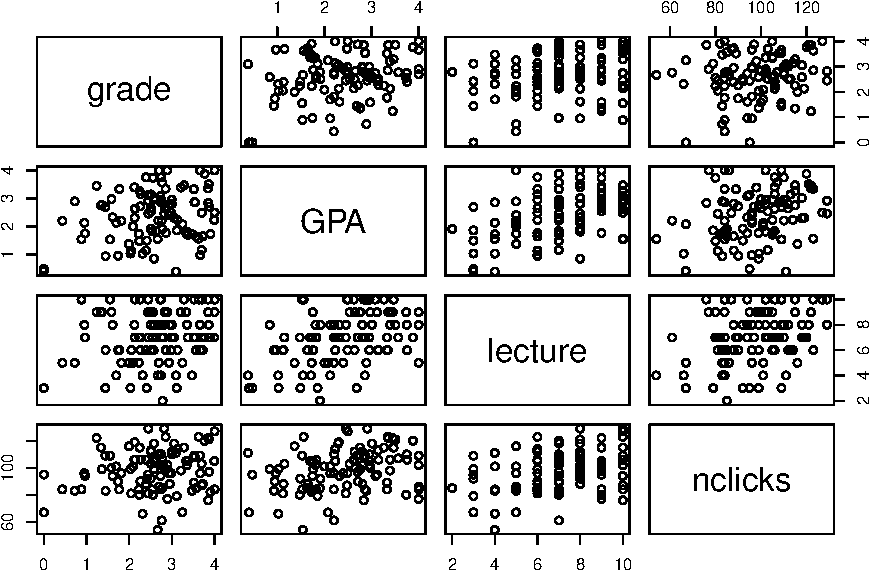
\includegraphics{L8_Multiple_regression_pdf_files/figure-latex/unnamed-chunk-4-1.pdf}

What can you infer from the correlation matrix?

\hypertarget{estimation-and-interpretation}{%
\section{Estimation and
interpretation}\label{estimation-and-interpretation}}

\begin{itemize}
\tightlist
\item
  For a Generalised Linear Model (GLM) with \(m\) predictors:
\end{itemize}

\[Y_i = \beta_0 + \beta_1 X_{1i} + \beta_2 X_{2i} + ... \beta_mX_{mi} + e_i\]

\begin{itemize}
\tightlist
\item
  Where\ldots{}

  \begin{itemize}
  \tightlist
  \item
    \(Y_i\) = the \emph{response variable} (or, the outcome to be
    predicted)
  \item
    \(\beta_0\) = the intercept term
  \item
    \(\beta_1 X_{1i}\) = the regression coefficient for predictor
    variable \(X_1\)
  \item
    \(\beta_2 X_{2i}\) = the regression coefficient for predictor
    variable \(X_2\)
  \item
    \(e_i\) = model residuals
  \item
    \(\hat{hat}\) = presence of a hat denotes and sample estimate, not
    the actual sample statistic
  \end{itemize}
\end{itemize}

\hypertarget{writing-out-the-formula-in-r}{%
\section{Writing out the formula in
R}\label{writing-out-the-formula-in-r}}

\begin{itemize}
\tightlist
\item
  Writing out a multiple regression model in R is much like what we did
  for simple regression, except you need to add a term for each
  predictor variable (\(X\)):
\end{itemize}

\begin{Shaded}
\begin{Highlighting}[]
\FunctionTok{lm}\NormalTok{(Y }\SpecialCharTok{\textasciitilde{}}\NormalTok{ X1 }\SpecialCharTok{+}\NormalTok{ X2 }\SpecialCharTok{+}\NormalTok{ ... }\SpecialCharTok{+}\NormalTok{ Xm, data)}
\end{Highlighting}
\end{Shaded}

\begin{itemize}
\tightlist
\item
  \textbf{Note}: You do not need to specify the intercept or the
  residuals, as these are included by default.
\end{itemize}

\hypertarget{predicting-grade-based-on-lecture-and-nclicks}{%
\section{\texorpdfstring{Predicting \texttt{grade} based on
\texttt{lecture} and
\texttt{nclicks}}{Predicting grade based on lecture and nclicks}}\label{predicting-grade-based-on-lecture-and-nclicks}}

\begin{Shaded}
\begin{Highlighting}[]
\NormalTok{my\_model }\OtherTok{\textless{}{-}} 
  \FunctionTok{lm}\NormalTok{(grade }\SpecialCharTok{\textasciitilde{}}\NormalTok{ lecture }\SpecialCharTok{+}\NormalTok{ nclicks, grades)}

\CommentTok{\# Summarise the model}
\FunctionTok{summary}\NormalTok{(my\_model)}
\end{Highlighting}
\end{Shaded}

\begin{verbatim}
## 
## Call:
## lm(formula = grade ~ lecture + nclicks, data = grades)
## 
## Residuals:
##      Min       1Q   Median       3Q      Max 
## -2.21653 -0.40603  0.02267  0.60720  1.38558 
## 
## Coefficients:
##             Estimate Std. Error t value Pr(>|t|)  
## (Intercept) 1.462037   0.571124   2.560   0.0120 *
## lecture     0.091501   0.045766   1.999   0.0484 *
## nclicks     0.005052   0.006051   0.835   0.4058  
## ---
## Signif. codes:  0 '***' 0.001 '**' 0.01 '*' 0.05 '.' 0.1 ' ' 1
## 
## Residual standard error: 0.8692 on 97 degrees of freedom
## Multiple R-squared:  0.06543,    Adjusted R-squared:  0.04616 
## F-statistic: 3.395 on 2 and 97 DF,  p-value: 0.03756
\end{verbatim}

\hypertarget{model-results}{%
\section{Model results}\label{model-results}}

\begin{itemize}
\tightlist
\item
  From the output, we can see that

  \begin{itemize}
  \tightlist
  \item
    \(\hat{\beta_0} = 1.46\) (intercept)
  \item
    \(\hat{\beta_1} = 0.09\) (\texttt{lecture} coefficient)
  \item
    \(\hat{\beta_2} = 0.01\) (\texttt{nclicks} coefficient)
  \end{itemize}
\end{itemize}

\hypertarget{plugging-the-estimates-back-into-the-formula}{%
\section{Plugging the estimates back into the
formula}\label{plugging-the-estimates-back-into-the-formula}}

\begin{itemize}
\tightlist
\item
  The result indicates that the following formula can be used to
  describe how a persons grade is predicted by their lecture attendance
  and course material download behaviour:
\end{itemize}

\texttt{grade} = 1.46 + 0.09 × \texttt{lecture} + 0.01 ×
\texttt{nclicks}

\begin{itemize}
\item
  And, because the regression coefficients of \(\hat{\beta_1}\)
  (\texttt{lecture}) and \(\hat{\beta_2}\) (\texttt{nclicks}) are both
  positive we can surmise that these predictors have a positive impact
  on \texttt{grade}.
\item
  If you had data on students \texttt{nclicks} and \texttt{lecture}
  attendance, you could use this to estimate their grade, based on the
  multiple regression model.
\end{itemize}

\hypertarget{predicting-from-new-data}{%
\section{Predicting from new data}\label{predicting-from-new-data}}

\begin{itemize}
\tightlist
\item
  \textbf{Warning}: If you want to pass new data to your multiple
  regression model the variable names have to match exactly. R is
  unforgiving when it comes to labels, so match sure both the name and
  text case is the same in your data and the model.
\end{itemize}

\begin{Shaded}
\begin{Highlighting}[]
\CommentTok{\# FYI: A \textquotesingle{}tribble\textquotesingle{} is a way to make a tibble by rows, rather than by columns}

\NormalTok{new\_data }\OtherTok{\textless{}{-}} 
  \FunctionTok{tribble}\NormalTok{(}\SpecialCharTok{\textasciitilde{}}\NormalTok{lecture, }\SpecialCharTok{\textasciitilde{}}\NormalTok{nclicks,}
          \DecValTok{3}\NormalTok{, }\DecValTok{70}\NormalTok{,}
          \DecValTok{10}\NormalTok{, }\DecValTok{130}\NormalTok{,}
          \DecValTok{0}\NormalTok{, }\DecValTok{20}\NormalTok{,}
          \DecValTok{5}\NormalTok{, }\DecValTok{100}\NormalTok{)}
\end{Highlighting}
\end{Shaded}

\begin{center}\rule{0.5\linewidth}{0.5pt}\end{center}

\begin{itemize}
\tightlist
\item
  Now that we've created our table \texttt{new\_data}, we can pass it to
  mutate and predict() to add a vector with the predictions for \(Y\)
  (\texttt{grade}).
\item
  Remember we have already created a model called
  \textbf{\texttt{my\_model}} based on the composition:
\end{itemize}

\texttt{lm(grade\ \textasciitilde{}\ lecture\ +\ nclicks,\ data\ =\ grades)}

\begin{Shaded}
\begin{Highlighting}[]
\CommentTok{\# Add predicted grade vector using \textasciigrave{}predict\textasciigrave{} function}
\NormalTok{new\_data }\SpecialCharTok{|\textgreater{}}
  \FunctionTok{mutate}\NormalTok{(}\AttributeTok{predicted\_grade =} \FunctionTok{predict}\NormalTok{(my\_model, new\_data))}
\end{Highlighting}
\end{Shaded}

\begin{verbatim}
## # A tibble: 4 x 3
##   lecture nclicks predicted_grade
##     <dbl>   <dbl>           <dbl>
## 1       3      70            2.09
## 2      10     130            3.03
## 3       0      20            1.56
## 4       5     100            2.42
\end{verbatim}

\hypertarget{visualising-partial-effects}{%
\section{Visualising Partial
effects}\label{visualising-partial-effects}}

\begin{itemize}
\tightlist
\item
  Each regression coefficient parameter estimate indicates the
  \emph{partial effect} of that variable; i.e., that variable's effect
  holding all other variables constant.
\item
  You can visualise partial effects using \texttt{predict} by

  \begin{itemize}
  \tightlist
  \item
    making a table with varying values of the focal predictor and
    filling all other predictors with their mean values (i.e., keep them
    constant)
  \end{itemize}
\end{itemize}

\hypertarget{visualising-the-partial-effect-of-lecture-on-grade-holding-nclicks-constant}{%
\section{\texorpdfstring{Visualising the partial effect of
\texttt{lecture} on \texttt{grade} holding \texttt{nclicks}
constant}{Visualising the partial effect of lecture on grade holding nclicks constant}}\label{visualising-the-partial-effect-of-lecture-on-grade-holding-nclicks-constant}}

\begin{itemize}
\tightlist
\item
  Remember, \texttt{lecture} is an integer from 0:10, so we want to
  create a vector that includes each of these levels.
\item
  To keep \texttt{nclicks} constant, let's create a vector that only
  contains the mean value for \texttt{nclicks}.
\end{itemize}

\hypertarget{r-code-for-partial-effects}{%
\subsection{R code for partial
effects}\label{r-code-for-partial-effects}}

\begin{Shaded}
\begin{Highlighting}[]
\CommentTok{\# Create vector containing nclicks mean}
\NormalTok{nclicks\_mean }\OtherTok{\textless{}{-}} 
\NormalTok{  grades }\SpecialCharTok{|\textgreater{}}         \CommentTok{\# take the grades dataset}
  \FunctionTok{pull}\NormalTok{(nclicks) }\SpecialCharTok{|\textgreater{}}  \CommentTok{\# extract single column from df as a vector}
  \FunctionTok{mean}\NormalTok{()}

\CommentTok{\# Create new data for prediction}
\NormalTok{new\_lecture }\OtherTok{\textless{}{-}} 
  \FunctionTok{tibble}\NormalTok{(}\AttributeTok{lecture =} \DecValTok{0}\SpecialCharTok{:}\DecValTok{10}\NormalTok{,         }\CommentTok{\# create vector containing each level of lecture}
         \AttributeTok{nclicks =}\NormalTok{ nclicks\_mean) }\CommentTok{\# add vector of nclicks mean}

\CommentTok{\# Add predicted grades vector controlling for effects of nclicks}
\NormalTok{new\_lecture2 }\OtherTok{\textless{}{-}} 
\NormalTok{  new\_lecture }\SpecialCharTok{|\textgreater{}}
  \FunctionTok{mutate}\NormalTok{(}\AttributeTok{grade =} \FunctionTok{predict}\NormalTok{(my\_model, new\_lecture))  }

\CommentTok{\# Present data}
\NormalTok{new\_lecture2}
\end{Highlighting}
\end{Shaded}

\begin{verbatim}
## # A tibble: 11 x 3
##    lecture nclicks grade
##      <int>   <dbl> <dbl>
##  1       0    98.3  1.96
##  2       1    98.3  2.05
##  3       2    98.3  2.14
##  4       3    98.3  2.23
##  5       4    98.3  2.32
##  6       5    98.3  2.42
##  7       6    98.3  2.51
##  8       7    98.3  2.60
##  9       8    98.3  2.69
## 10       9    98.3  2.78
## 11      10    98.3  2.87
\end{verbatim}

\hypertarget{plot-partial-effets}{%
\section{Plot Partial effets}\label{plot-partial-effets}}

\begin{Shaded}
\begin{Highlighting}[]
\CommentTok{\# Plot partial effect of lecture on grade}
\CommentTok{\# Holding \textasciigrave{}nclicks\textasciigrave{} constant}
\FunctionTok{ggplot}\NormalTok{(grades, }\FunctionTok{aes}\NormalTok{(lecture, grade)) }\SpecialCharTok{+} 
  \FunctionTok{geom\_point}\NormalTok{() }\SpecialCharTok{+}
  \FunctionTok{geom\_line}\NormalTok{(}\AttributeTok{data =}\NormalTok{ new\_lecture2) }\SpecialCharTok{+} \CommentTok{\# add your }
  \FunctionTok{labs}\NormalTok{(}\AttributeTok{title =} \StringTok{"Partial effect of lecture on grade."}\NormalTok{, }
       \AttributeTok{x =} \StringTok{"Lectures attended"}\NormalTok{,}
       \AttributeTok{y =} \StringTok{"Predicted grade"}\NormalTok{)}
\end{Highlighting}
\end{Shaded}

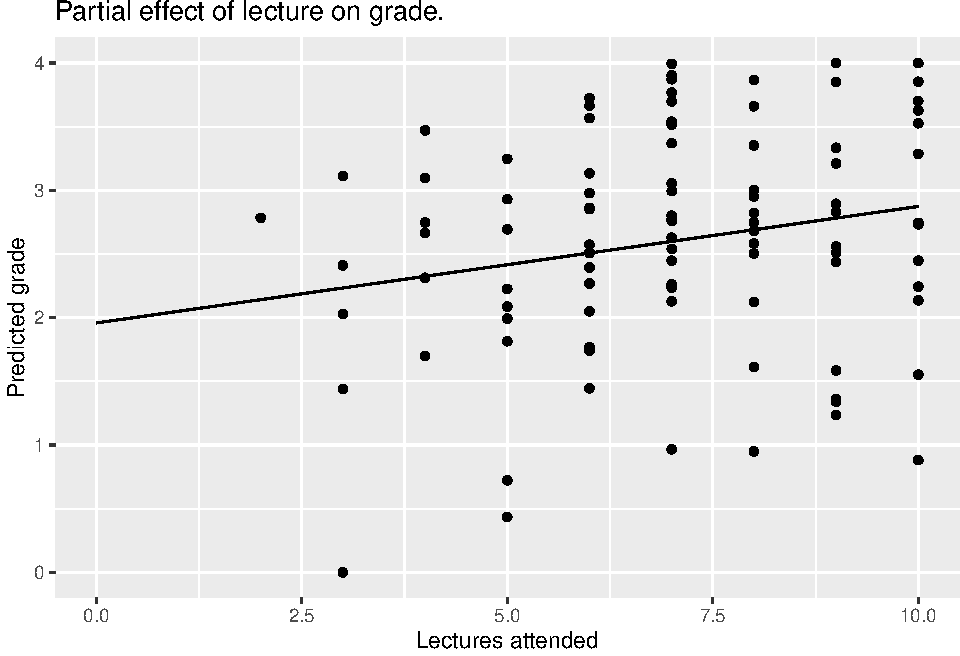
\includegraphics{L8_Multiple_regression_pdf_files/figure-latex/unnamed-chunk-10-1.pdf}

\hypertarget{a-word-on-partial-effects-plots}{%
\subsection{A word on partial effects
plots}\label{a-word-on-partial-effects-plots}}

\begin{itemize}
\tightlist
\item
  Partial effects plots are meaningful when there are no interactions in
  the model between the focal predictor and any other predictors.
\item
  This is because, when there are interactions, the partial effect of a
  focal predictor \(X_i\) will differ across the values of other
  predictors it interacts with.
\end{itemize}

\hypertarget{standardising-coefficients}{%
\section{Standardising Coefficients}\label{standardising-coefficients}}

\begin{itemize}
\tightlist
\item
  Part of multiple regression modelling is determining which of the
  predictors in your model matter the most when predicting \(Y\).
\item
  In the analysis above, all of the \(\hat{\beta}\) (coefficient
  estimates) come from different scales, so comparing their values is
  meaningless.
\item
  One way you can convert these scales into something comparable is to
  convert them into \textbf{z-scores}.
\end{itemize}

\[z = \frac{X - \mu_x}{\sigma_x}\]

\hypertarget{z-scores}{%
\subsection{Z-scores}\label{z-scores}}

\begin{itemize}
\tightlist
\item
  z-scores represent how far a value of \(X\) is from the sample mean
  (\(\mu_x\)) in standard deviations (\(\sigma_x\)).
\item
  When you re-scale using z-scores the mean of the scale is set to 0.
\item
  So, a z-score of 1 (\(z = 1\)) means that that particular score for
  \(X\) is one standard deviation higher than the mean, and -1 would
  indicate a score 1 standard deviation below the mean.
\item
  Z-scores offer a means to compare data that come from different
  populations by converting the values to a standard normal distribution
  (a distribution with a mean of 0 and SD = 1).
\end{itemize}

\hypertarget{rescaling-predictors}{%
\section{Rescaling predictors}\label{rescaling-predictors}}

\begin{Shaded}
\begin{Highlighting}[]
\CommentTok{\# Create new object with scaled z{-}score data vectors}
\NormalTok{grades2 }\OtherTok{\textless{}{-}} 
\NormalTok{  grades }\SpecialCharTok{|\textgreater{}}
  \FunctionTok{mutate}\NormalTok{(}\AttributeTok{lecture\_c =} 
\NormalTok{           (lecture }\SpecialCharTok{{-}} \FunctionTok{mean}\NormalTok{(lecture)) }\SpecialCharTok{/} \FunctionTok{sd}\NormalTok{(lecture), }\CommentTok{\# apply z{-}score formula}
         \AttributeTok{nclicks\_c =} 
\NormalTok{           (nclicks }\SpecialCharTok{{-}} \FunctionTok{mean}\NormalTok{(nclicks)) }\SpecialCharTok{/} \FunctionTok{sd}\NormalTok{(nclicks))}

\CommentTok{\# Examine the data}
\FunctionTok{head}\NormalTok{(grades2)}
\end{Highlighting}
\end{Shaded}

\begin{verbatim}
## # A tibble: 6 x 6
##   grade   GPA lecture nclicks lecture_c nclicks_c
##   <dbl> <dbl>   <int>   <int>     <dbl>     <dbl>
## 1  2.40 1.13        6      88    -0.484   -0.666 
## 2  3.67 0.971       6      96    -0.484   -0.150 
## 3  2.85 3.34        6     123    -0.484    1.59  
## 4  1.36 2.76        9      99     0.982    0.0439
## 5  2.31 1.02        4      66    -1.46    -2.09  
## 6  2.58 0.841       8      99     0.493    0.0439
\end{verbatim}

\begin{center}\rule{0.5\linewidth}{0.5pt}\end{center}

\begin{itemize}
\tightlist
\item
  Now let's fit a model using our z-scores for equal comparison
\end{itemize}

\begin{Shaded}
\begin{Highlighting}[]
\NormalTok{my\_model\_scaled }\OtherTok{\textless{}{-}} 
  \FunctionTok{lm}\NormalTok{(grade }\SpecialCharTok{\textasciitilde{}}\NormalTok{ lecture\_c }\SpecialCharTok{+}\NormalTok{ nclicks\_c, }
\NormalTok{     grades2)}

\CommentTok{\# Summarise the model}
\FunctionTok{summary}\NormalTok{(my\_model\_scaled)}
\end{Highlighting}
\end{Shaded}

\begin{verbatim}
## 
## Call:
## lm(formula = grade ~ lecture_c + nclicks_c, data = grades2)
## 
## Residuals:
##      Min       1Q   Median       3Q      Max 
## -2.21653 -0.40603  0.02267  0.60720  1.38558 
## 
## Coefficients:
##             Estimate Std. Error t value            Pr(>|t|)    
## (Intercept)  2.59839    0.08692  29.895 <0.0000000000000002 ***
## lecture_c    0.18734    0.09370   1.999              0.0484 *  
## nclicks_c    0.07823    0.09370   0.835              0.4058    
## ---
## Signif. codes:  0 '***' 0.001 '**' 0.01 '*' 0.05 '.' 0.1 ' ' 1
## 
## Residual standard error: 0.8692 on 97 degrees of freedom
## Multiple R-squared:  0.06543,    Adjusted R-squared:  0.04616 
## F-statistic: 3.395 on 2 and 97 DF,  p-value: 0.03756
\end{verbatim}

\hypertarget{interpretation}{%
\section{Interpretation}\label{interpretation}}

\begin{itemize}
\tightlist
\item
  Now that we have scaled the data we can compare the coefficient
  estimates
\item
  The model output indicates that \texttt{lecture\_c} actually had more
  of an impact on \texttt{grade}, with each SD increase in lecture\_c
  grade increased by 0.19 (i.e., \(\hat{\beta_1}=0.19\)).
\item
  This is compared to our un-scaled model where the estimate was 0.091
  (i.e., \(\hat{\beta_1}=0.09\))
\end{itemize}

\hypertarget{model-comparison}{%
\section{Model Comparison}\label{model-comparison}}

\begin{itemize}
\tightlist
\item
  You may also want to check whether a predictor variable significantly
  affects the dependent (or response) variable, over and above the
  effect of one of your control variables.
\item
  We saw above that the model including \texttt{lecture} and
  \texttt{nclicks} was significant, \(F(2,97) = 3.395, p = 0.038\).
\end{itemize}

\begin{itemize}
\tightlist
\item
  The null hypothesis for a multiple regression model represents a model
  where all of the coefficients (other than the intercept) are zero:
  \(H_0 : \beta_1 - \beta_2 = ... = \beta_m = 0\) OR \(Y_i = \beta_0\)
\item
  Put differently, your best prediction of \(Y\) is simply its mean
  (\(\mu_y\)), and the \(X\) predictor variables have no effect on
  \(Y\).
\item
  The regression model above rejects \(H_0\), indicating that
  \texttt{lecture} and \texttt{nclicks} can be used to predict
  \texttt{grade}.
\end{itemize}

\hypertarget{reconceptualising-the-question}{%
\section{Reconceptualising the
question}\label{reconceptualising-the-question}}

\begin{itemize}
\tightlist
\item
  It is possible that better students (who are more likely to attend
  lectures and download online course content) are simply more likely to
  get better grades.
\item
  If this is true, than the relationship between \texttt{lecture},
  \texttt{nclicks}, and \texttt{grade} would be mediated by student
  quality.
\item
  So, the question becomes; \textbf{are \texttt{lecture} and
  \texttt{nclicks} associated with better grades above and beyond
  student ability, indicated by \texttt{GPA}}.
\end{itemize}

\hypertarget{running-model-comparisons}{%
\section{Running model comparisons}\label{running-model-comparisons}}

\begin{enumerate}
\def\labelenumi{\arabic{enumi}.}
\tightlist
\item
  Estimate a model containing any control predictors, excluding the
  focal predictors.
\item
  Estimate a model containing the control predictors, including the
  focal predictors.
\item
  Compare the two models using \texttt{anova}
\end{enumerate}

\hypertarget{r-code-for-model-comparisons}{%
\section{R Code for model
comparisons}\label{r-code-for-model-comparisons}}

\begin{Shaded}
\begin{Highlighting}[]
\CommentTok{\# Control model}
\NormalTok{m1 }\OtherTok{\textless{}{-}} 
  \FunctionTok{lm}\NormalTok{(grade }\SpecialCharTok{\textasciitilde{}}\NormalTok{ GPA, grades) }

\CommentTok{\# Focal predictor model}
\NormalTok{m2 }\OtherTok{\textless{}{-}} 
  \FunctionTok{lm}\NormalTok{(grade }\SpecialCharTok{\textasciitilde{}}\NormalTok{ GPA }\SpecialCharTok{+}\NormalTok{ lecture }\SpecialCharTok{+}\NormalTok{ nclicks, grades) }

\CommentTok{\# Run the model comparison}
\FunctionTok{anova}\NormalTok{(m1, m2)}
\end{Highlighting}
\end{Shaded}

\begin{verbatim}
## Analysis of Variance Table
## 
## Model 1: grade ~ GPA
## Model 2: grade ~ GPA + lecture + nclicks
##   Res.Df    RSS Df Sum of Sq      F Pr(>F)
## 1     98 73.528                           
## 2     96 71.578  2    1.9499 1.3076 0.2752
\end{verbatim}

\hypertarget{interpretation-of-model-comparisons}{%
\section{Interpretation of model
comparisons}\label{interpretation-of-model-comparisons}}

\begin{itemize}
\tightlist
\item
  \(H_0\) states that we can predict \texttt{grade} from \texttt{GPA},
  just as well as we can from \texttt{GPA}, \texttt{lecture}, and
  \texttt{nclicks}.
\item
  \(H_0\) will be rejected if the inclusion of \texttt{lecture} and
  \texttt{nclicks} (i.e., in the focal predictor model) leads to a
  substantial reduction in the residual sum of squares.
\item
  This would indicate that their inclusion helps to signidicantly reduce
  the amount of unexplained variance in the model.
\item
  The result \(F(2,96) = 1.308, p = 0.275\) shows that our control
  variable model is as good at explaining the results as our focal
  predictor model.
\item
  So, \texttt{lecture} and \texttt{nclicks} do not predict better grades
  more so than \texttt{GPA} alone.
\end{itemize}

\hypertarget{what-did-we-cover-today}{%
\section{What did we cover today}\label{what-did-we-cover-today}}

\begin{itemize}
\tightlist
\item
  Equations/formula for multiple regression
\item
  Worked example using the ``grades.csv'' dataset from PsyTeachR
\item
  The \texttt{predict} function
\item
  Calculating and visualising partial effects
\item
  Comparing standard models and non-standardised models
\end{itemize}

\hypertarget{tutorial-exercise-for-this-week}{%
\section{Tutorial exercise for this
week}\label{tutorial-exercise-for-this-week}}

\begin{itemize}
\tightlist
\item
  Visualize the partial effect of \texttt{nclicks} on \texttt{grade}.
\end{itemize}

\hypertarget{reading}{%
\section{Reading}\label{reading}}

\href{https://psyteachr.github.io/stat-models-v1/multiple-regression.html}{Learning
Statistical Models Through Simulation in R: Chapter 4 Multiple
Regression}

\end{document}
